
\chapter{Using this class}

\section{Dependencies}

Here are the packages already loaded, so there is no need to re-include them in your document:

\begin{wide}\setstretch{1.0}
	\begin{multicols}{4}
		\begin{itemize}
			\item\texttt{geometry}
			\item\texttt{emptypage}
			\item\texttt{fullwidth}
			\item\texttt{sidenotes}
			\item\texttt{caption}
			\item\texttt{fontenc}
			\item\texttt{libertinus}
			\item\texttt{libertinust1math}
			\item\texttt{gillius}
			\item\texttt{droidsansmono}
			\item\texttt{ragged2e}
			\item\texttt{titlesec}
			\item\texttt{titletoc}
			\item\texttt{tocloft}
			\item\texttt{fancyhdr}
			\item\texttt{graphicx} \item\texttt{microtype} \item\texttt{amsfonts} \item\texttt{amsmath} \item\texttt{mathtools} \item\texttt{physics} \item\texttt{xcolor} \item\texttt{mdframed} \item\texttt{tabularx} \item\texttt{booktabs} \item\texttt{enumitem} \item\texttt{hyperref} \item\texttt{etoolbox} \item\texttt{changepage} \item\texttt{placeins} \item\texttt{xparse} \item\texttt{xpatch} \item\texttt{biblatex} \item\texttt{listings}
		\end{itemize}
	\end{multicols}
\end{wide}

\section{The big margin}

There is a big margin, so feel free to use it as much as possible!\footnote{Actually to your needs, if you do not have a natural usage of notes, maybe do not use this class.\\By the way, see how sidenote numbers reset on new chapters: we're back on number 1!} This chapter will cover the usage of sidenotes, side references, and other ways to use the margin.\footnote{For float captions, see chapter \ref{chp:floats}.}

The general layout is done using the \texttt{geometry}\sidecite{pkgGeometry} package, and all the margin stuff relies on the \texttt{sidenotes}\sidecite{pkgSidenotes} package, so check its documentation:

\bgroup
\centering\url{http://www.ctan.org/pkg/sidenotes}\RaggedRight\noindent for more in-depth information. \egroup

\subsection{Sidenotes}

To put a sidenote in the margin, use
\begin{codebox}{tex}
	\sidenote[<number>][<offset>]{<sidenote text>}
\end{codebox}
\begin{itemize}
	\item
	      \inlinecode{tex}{<number>} is an optional parameter for the sidenote number. For example, \inlinecode{tex}_\sidenote[29100][]{The sidenote.}_ does this.\sidenote[29100][]{The sidenote.}
	\item
	      \inlinecode{tex}{<offset>} is an offset length (in pt, px, en, em\dots) to vertically offset the sidenote. A positive value will have it go down, a negative go up.
\end{itemize}

\LaTeX{} natively allows to put unformatted content in the margin with the command \inlinecode{tex}_\marginpar{<your content>}_,\marginpar{This is unformatted margin text, in fullsize.} but I advise not to use it, as it puts raw fullsize text in the margin, and does not blend well with the overall design. Instead, use\sidetext{This is just some unnumbered piece of text in the margin, but with the formatting done right.}
\begin{codebox}{tex}
	\sidetext{<your text>}
\end{codebox}
This will format the margin text to match the sidenotes style.


\subsection{Side references}

The margin is also handy to put bibliographic references:\sidecite{einstein1915allgemeinen} the reader can read them directly instead of going all through the document to find the right entry in the references section. But don't worry, each reference displayed in the margin is labelled with a number and appears in a dedicated bibliography section. All in all, a side reference is displayed in the margin in a shortened form, and then again in the bibliography in the full form.

To cite a paper, use
\begin{codebox}{tex}
	\sidecite{<reference label>}
\end{codebox}


\section{Full width text}

\begin{wide}
	It may be handy to have the text span the whole page width, like this paragraph. Use the environment \inlinecode{tex}_\begin{wide}...\end{wide}_ to do this. It should manage page breaks properly, but it is not optimal: no not use it for too long (like for ten pages), the behavior tends to go a little wild. The behavior of \inlinecode{tex}{\sidenote}, \inlinecode{tex}{\marginpar} and \inlinecode{tex}{\sidecite} is not supported in the \inlinecode{tex}{wide} environment.

	Also, for floating environments, full width figures and tables will be covered in the chapter \ref{chp:floats}, so do not use the \inlinecode{tex}{wide} environments with figures or tables (actually tables are fine, but there are specific environments for them to be in full width).
\end{wide}

\section{The skeleton}

The structure of a \LaTeX{} book is as follows:
\begin{codebox}{tex}
	% preamble
\begin{document}

\maketitle % titlepage

\frontmatter % unnumbered preliminary chapters
\chapter{}
\tableofcontents

\mainmatter % main content: numbered chapters
\part{part}
\chapter{content}
\chapter{content}

\appendix % letter numbered chapters
\chapter{appendix 1}
\chapter{appendix 2}

\backmatter % everything else: references, indexes, glossaries, etc.
\printbibliography
\printindex

\end{document}
\end{codebox}

\subsection{The new \texttt{\textbackslash maketitle}}

The \inlinecode{tex}_\maketitle_ macro has been slightly pimped up. It now displays a custom titlepage ---like the one on this very document, as well as a copyright tag, a dedication word and a colophon.

\section{Floats}
\label{chp:floats}

The integration of floats with the Tufte layout is handled with the \texttt{sidenotes} package, loaded with the class definition. The following paragraphs show how to basically use the macros, and for more information, see the package documentation at \url{https://www.ctan.org/pkg/sidenotes}.

\subsection{Figures}

Edward Tufte's designs are known to be really tight when it comes to including images with text. The main pet peeve I had with one-column designs is when I included a small figure in the document, it had to visually break the text and generate large unpleasing blank spaces. Also, more often than not, the text width was too much for the images, resulting in huge one-liner captions for very small figures.

The 1.5-column design fixes this by putting all captions in the margins, as well as small enough figures, which tidies the document a lot.

\textfig[1]{figures/bretagne.png}{1919 map of the Finistère in French Brittany. This figure is in the main text column, with a caption in the margin aligned with the top of the image. For images narrower than the text width, they will be outer-aligned so that they remain just next their caption.}{fig:figure-text}

% \begin{figure}[htbp]
% 	\sidecaption{1919 map of the Finistère in French Brittany. This figure is in the main text column, with a caption in the margin aligned with the top of the image. For images with width less than the text width, they will be outer-aligned so that they are close to the caption.}\label{fig:figure-text}
% 	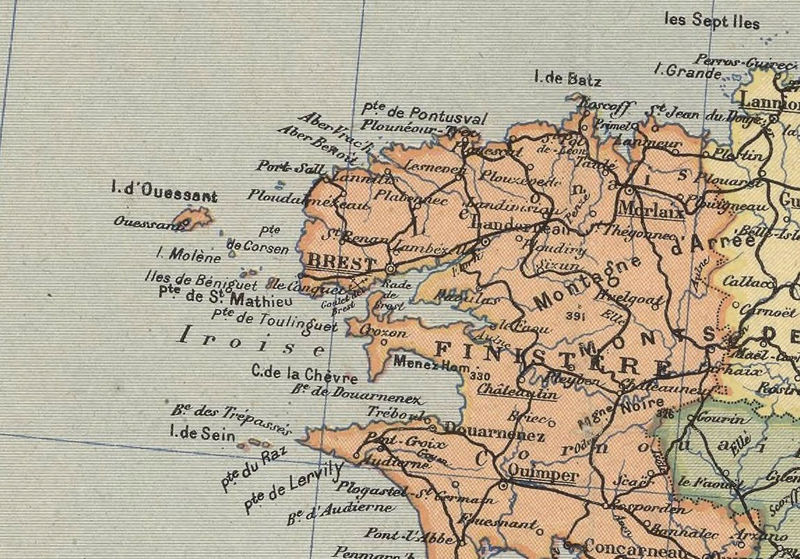
\includegraphics[width = \linewidth, outer]{figures/bretagne.png}
% \end{figure}


To put a graphics in the text like in the figure \ref{fig:figure-text}, use\footnote{The \texttt{\textbackslash label} \textit{has} to be inside the \texttt{\textbackslash sidecaption} command, otherwise references with \texttt{\textbackslash ref} won't work.}

\begin{codebox}{tex}
    \begin{figure}
        \sidecaption{<caption>\label{<label>}} % put this on top
        % \label HAS to be inside the \sidecaption
        \includegraphics[]{<>} % or tikz or anything
    \end{figure}
\end{codebox}


To put a figure in the margin like the figure \ref{fig:figure-margin}, use

\begin{codebox}{tex}
\begin{marginfigure}
\includegraphics[]{<>} % or tikz or anything
\caption{<caption>\label{<label>}}
\end{figure}
\end{codebox}

\marginfig{figures/marine-knots.jpg}{The most common sea boat knots. This image can be displayed rather small, so it fits in the margin. The caption is displayed below.}{fig:figure-margin}

For wide figures like the figure \ref{fig:figure-fullwidth}, use

\begin{codebox}{tex}
    \begin{figure*}
        \includegraphics[]{<>} % or tikz or anything
        \sidecaption{<caption>\label{<label>}}
    \end{figure*}
\end{codebox}

\newpage

\widefig{figures/usa-census.png}{The US census map from data collected in 2010 -- \url{www.ecpmlangues.u-strasbg.fr}\\This is a wide figure, stretching from the innermost to the outermost margin.}{fig:figure-fullwidth}


\subsection{Shortcuts}

I find typing figure environments repetitive for long (even short) documents, so I made the following macro for figures with \texttt{\textbackslash sidecaption}s :

\begin{codebox}{tex}
    \textfig[<optional width>]{<file path>}{<caption>}{<label>}
\end{codebox}

The \inlinecode{}{<optional width>} is a number between zero and one wich determines the image width relative to the text width. The default value is 1, like on the figure \ref{fig:figure-text}.

The same macros are provided for images in the magins and wide images, respectively shown in figures \ref{fig:figure-margin} and \ref{fig:figure-fullwidth}.

\begin{codebox}{tex}
    % figure in the margin
    \marginfig[<optional width>]{<file path>}{<caption>}{<label>}
    % wide figure
    \widefig[<optional width>]{<file path>}{<caption>}{<label>}
\end{codebox}



If for any reason a figure caption has to be put in the main text block, just use the regular \texttt{figure} environment. The following shortcut macros will also do. The result of \inlinecode{tex}{\plainfig} is shown in figure \ref{fig:figure-plain}.

\begin{codebox}{tex}
    % plain figure with textwidth
    \plainfig[<optional width>]{<file path>}{<caption>}{<label>}
    % plain figure with full width
    \plainwidefig[<optional width>]{<file path>}{<caption>}{<label>}
\end{codebox}

% \plainfig[.7]{figures/mandelbrot.png}{The Mandelbrot set with different depths of iteration. This caption is not in the margin but in the main text area. It can sometimes be useful with really really long captions. \lipsum[1]}{fig:figure-plain}

\begin{figure}[htb!]
    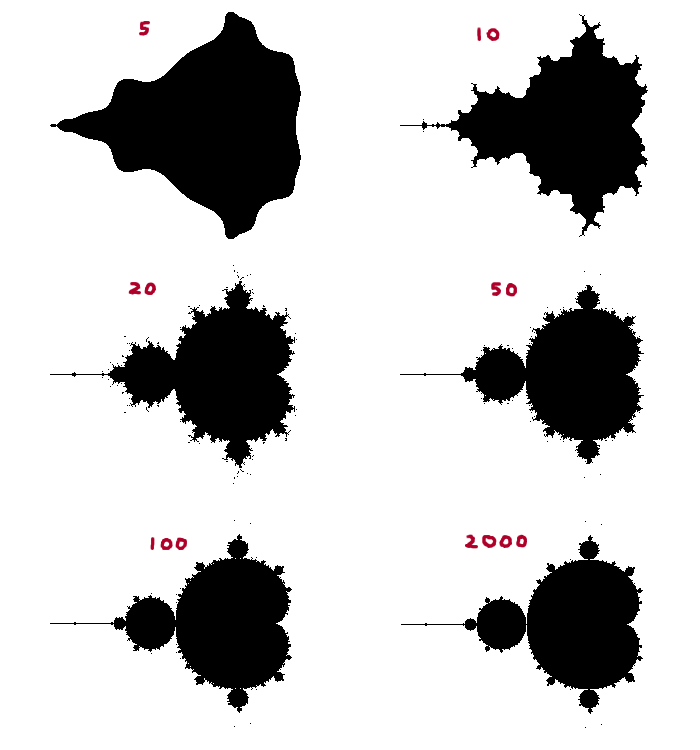
\includegraphics[width =.7\linewidth]{figures/mandelbrot.png}
    \caption[The Mandelbrot set with different depths of iteration. This caption is not in the margin but in the main text area. It can sometimes be useful with really really long captions.]{The Mandelbrot set with different depths of iteration. This caption is not in the margin but in the main text area. It can sometimes be useful with really really long captions. \lipsum[1]\label{fig:figure-plain}}

\end{figure}

\newpage
\subsection{Tables}

Table environments work the same as figures, as is is shown in tables \ref{tab:table-text} and \ref{tab:table-wide}.

\begin{table}[!htb]\small
    \sidecaption{The elementary particles included in the standard model. This is a table with a \texttt{\textbackslash sidecaption}.\label{tab:table-text}}
    \begin{tabular}{lllll}
        \multicolumn{5}{l}{\textbf{The Standard model of Elementary Particles.}}                                                                                                                                                               \\
        \toprule
        \multicolumn{3}{l}{\textbf{Three generations of matter (fermions)}} & \multicolumn{2}{l}{\textbf{Interactions (bosons)}}                                                                                                               \\
        I                                                                   & II                                                    & III                                                    &                             &                   \\
        % \cmidrule(lr){1-3}\cmidrule(lr){4-5}
        \multicolumn{3}{c}{\textsc{quarks}}                                 & \textsc{gauge}                                        & \textsc{scalar}                                                                                          \\
        \cmidrule(lr){1-3}\cmidrule(lr){4-4}\cmidrule(lr){5-5}
        \textbf{u}~~up                                                      & \textbf{c}~~charm                                     & \textbf{t}~~top                                        & \textbf{g}~~gluon           & \textbf{H}~~higgs \\
        \textbf{d}~~down                                                    & \textbf{s}~~strange                                   & \textbf{b}~~bottom                                     & \textbf{\textgamma}~~photon &                   \\
        \multicolumn{3}{c}{\textsc{leptons}}                                & \textbf{Z} boson                                      &                                                                                                          \\
        \cmidrule(lr){1-3}
        \textbf{e}~~electron                                                & \textbf{\textmu}~~muon                                & \textbf{\texttau}~~tau                                 & \textbf{W} boson            &                   \\
        \textbf{\textnu\textsubscript{e}}~~el. neutrino                     & \textbf{\textnu\textsubscript{\textmu}}~~mu. neutrino & \textbf{\textnu\textsubscript{\texttau}}~~tau neutrino &                             &                   \\
        \bottomrule
    \end{tabular}
\end{table}


\begin{table*}[!htb]\small\sffamily
    \begin{tabularx}{\linewidth}{rXXXXXXrXXXXXX}
        \multicolumn{14}{l}{\textbf{Table des marées au port de Douarnenez (Finistère).}}                                                                                                                                                                                                                             \\
        \toprule
                    & \multicolumn{3}{c}{\textbf{Ven. 23 juillet 2021}} & \multicolumn{3}{c}{\textbf{Sam. 24 juillet 2021}} &       & \multicolumn{3}{c}{\textbf{Dim. 25 juillet 2021}} & \multicolumn{3}{c}{\textbf{Lun. 26 juillet 2021}}                                                                           \\
                    & heure                                             & hauteur                                           & coef. & heure                                             & hauteur                                           & coef. &             & heure & hauteur & coef. & heure & hauteur & coef. \\
        \cmidrule(lr){2-4}\cmidrule(lr){5-7}\cmidrule(lr){9-11}\cmidrule(lr){12-14}
        \textsc{bm} & 04:54                                             & 6.06                                              & 81    & 05:46                                             & 6.24                                              & 88    & \textsc{pm} & 00:21 & 0.92    & --    & 01:08 & 0.88    & --    \\
        \textsc{pm} & 11:05                                             & 1.38                                              & --    & 11:55                                             & 1.19                                              & --    & \textsc{bm} & 06:34 & 6.34    & 92    & 07:19 & 6.33    & 92    \\
        \textsc{bm} & 17:17                                             & 6.39                                              & 85    & 18:06                                             & 6.59                                              & 91    & \textsc{pm} & 12:41 & 1.10    & --    & 13:26 & 1.12    & --    \\
        \textsc{pm} & 23:33                                             & 1.10                                              & --    & ---:---                                           & --                                                & --    & \textsc{bm} & 18:52 & 6.67    & 93    & 19:36 & 6.63    & 91    \\
        \bottomrule
    \end{tabularx}
    \sidecaption{%
        Table des marées à Douarnenez du 23 au 26 juillet 2021, Service Hydrographique et Océanographique de la Marine, \url{maree.shom.fr}.\\This is a wide table, called with the \texttt{table*} environment. The caption is also a \texttt{\textbackslash sidecaption}.\label{tab:table-wide}
    }
\end{table*}

To typeset the table \ref{tab:table-text}, use the following code, which is just a \inlinecode{tex}_table_ environment with a \inlinecode{tex}_\sidecaption_. For table \ref{tab:table-wide}, use the \inlinecode{tex}_table*_ environment with either \inlinecode{tex}_\sidecaption_ or \inlinecode{tex}_\caption_.\inlinecode{tex}_\FloatBarrier_ is there to make sure the floats appear in order.
\sidenote[][100pt]{\texttt{\textbackslash FloatBarrier} works for all floating environments, including figures.}


\begin{codebox}{tex}
    \begin{table}[!htb]\small
        \sidecaption{The elementary particles included in the standard model. This is a table with a \texttt{\textbackslash sidecaption}.\label{tab:table-text}}
        \begin{tabular}{lllll}
            \multicolumn{5}{l}{\textbf{The Standard model of Elementary Particles.}}                                                                                                                                                               \\
            \toprule
            \multicolumn{3}{l}{\textbf{Three generations of matter (fermions)}} & \multicolumn{2}{l}{\textbf{Interactions (bosons)}}                                                                                                               \\
            I                                                                   & II                                                    & III                                                    &                             &                   \\
            \multicolumn{3}{c}{\textsc{quarks}}                                 & \textsc{gauge}                                        & \textsc{scalar}                                                                                          \\
            \cmidrule(lr){1-3}\cmidrule(lr){4-4}\cmidrule(lr){5-5}
            \textbf{u}~~up                                                      & \textbf{c}~~charm                                     & \textbf{t}~~top                                        & \textbf{g}~~gluon           & \textbf{H}~~higgs \\
            \textbf{d}~~down                                                    & \textbf{s}~~strange                                   & \textbf{b}~~bottom                                     & \textbf{\textgamma}~~photon &                   \\
            \multicolumn{3}{c}{\textsc{leptons}}                                & \textbf{Z} boson                                      &                                                                                                          \\
            \cmidrule(lr){1-3}
            \textbf{e}~~electron                                                & \textbf{\textmu}~~muon                                & \textbf{\texttau}~~tau                                 & \textbf{W} boson            &                   \\
            \textbf{\textnu\textsubscript{e}}~~el. neutrino                     & \textbf{\textnu\textsubscript{\textmu}}~~mu. neutrino & \textbf{\textnu\textsubscript{\texttau}}~~tau neutrino &                             &                   \\
            \bottomrule
        \end{tabular}
    \end{table}
\end{codebox}

\begin{codebox}{tex}
    \begin{table*}[!htb]\small\sffamily
        \begin{tabularx}{\linewidth}{rXXXXXXrXXXXXX}
            \multicolumn{14}{l}{\textbf{Table des marees au port de Douarnenez (Finistere).}}                                                                                                                                                                                                                             \\
            \toprule
                        & \multicolumn{3}{c}{\textbf{Ven. 23 juillet 2021}} & \multicolumn{3}{c}{\textbf{Sam. 24 juillet 2021}} &       & \multicolumn{3}{c}{\textbf{Dim. 25 juillet 2021}} & \multicolumn{3}{c}{\textbf{Lun. 26 juillet 2021}}                                                                           \\
                        & heure                                             & hauteur                                           & coef. & heure                                             & hauteur                                           & coef. &             & heure & hauteur & coef. & heure & hauteur & coef. \\
            \cmidrule(lr){2-4}\cmidrule(lr){5-7}\cmidrule(lr){9-11}\cmidrule(lr){12-14}
            \textsc{bm} & 04:54                                             & 6.06                                              & 81    & 05:46                                             & 6.24                                              & 88    & \textsc{pm} & 00:21 & 0.92    & --    & 01:08 & 0.88    & --    \\
            \textsc{pm} & 11:05                                             & 1.38                                              & --    & 11:55                                             & 1.19                                              & --    & \textsc{bm} & 06:34 & 6.34    & 92    & 07:19 & 6.33    & 92    \\
            \textsc{bm} & 17:17                                             & 6.39                                              & 85    & 18:06                                             & 6.59                                              & 91    & \textsc{pm} & 12:41 & 1.10    & --    & 13:26 & 1.12    & --    \\
            \textsc{pm} & 23:33                                             & 1.10                                              & --    & ---:---                                           & --                                                & --    & \textsc{bm} & 18:52 & 6.67    & 93    & 19:36 & 6.63    & 91    \\
            \bottomrule
        \end{tabularx}
        \sidecaption{%
            %
        }
    \end{table*}\FloatBarrier
\end{codebox}

To produce tables in the margin like table \ref{tab:table-margin}, use the \inlinecode{tex}{margintable} environment like in the following.

\begin{margintable}[0pt]\small
    \caption{Major, minor and perfect music intervals. ST. stands for \textit{semitones}. This table is in the margin. \label{tab:table-margin}}
    \begin{tabular}{ll}
        \toprule
        \textbf{ST.} & \textbf{Intervals}                                      \\
        \midrule
        0            & unison                                                  \\
        1            & minor second                                            \\
        2            & major second                                            \\
        3            & minor third                                             \\
        4            & major third                                             \\
        5            & perfect fourth                                          \\
        6            & aug. 4\textsuperscript{th} / dim. 5\textsuperscript{th} \\
        7            & perfect fifth                                           \\
        8            & minor sixth                                             \\
        9            & major sixth                                             \\
        10           & minor seventh                                           \\
        11           & major seventh                                           \\
        12           & octave                                                  \\
        \bottomrule
    \end{tabular}
\end{margintable}

\begin{codebox}{tex}
    \begin{margintable}[]\small
        \caption{Major, minor and perfect music intervals. ST. stands for \textit{semitones}. This table is in the margin. \label{tab:table-margin}}
        \begin{tabular}{ll}
            \toprule
            \textbf{ST.} & \textbf{Intervals}                                      \\
            \midrule
            0            & unison                                                  \\
            1            & minor second                                            \\
            2            & major second                                            \\
            3            & minor third                                             \\
            4            & major third                                             \\
            5            & perfect fourth                                          \\
            6            & aug. 4\textsuperscript{th} / dim. 5\textsuperscript{th} \\
            7            & perfect fifth                                           \\
            8            & minor sixth                                             \\
            9            & major sixth                                             \\
            10           & minor seventh                                           \\
            11           & major seventh                                           \\
            12           & octave                                                  \\
            \bottomrule
        \end{tabular}
    \end{margintable}
\end{codebox}


\subsection{Code}
\label{sub:code}

Code can be inserted, whether with simple code boxes or captioned snippets that look like the following.
\begin{snippet}{c}{Hello world in C. This is a captioned code snippet.}{snp:hello-world}
    int main(int argc, char *argv[]) {
            printf("Hello world!");
            return 0;
        }
\end{snippet}

The box is a light gray hairline that helps make the code stick out just enough without distracting the eye too much. The code itself is syntax colored according to the used language. There are several environments for code boxes, explained below.

For a simple code box with neither line numbering nor caption, the macro environment is the following.

\sidetext{%
    This supports most of the classic languages. Here are some examples for the language option:

    \inlinecode{}{c},

    \indent\inlinecode{}{c++},

    \indent\inlinecode{}{python},

    \indent\inlinecode{}{java},

    \indent\inlinecode{}{latex}\dots\\
    If a specific language is not recognized, use the \inlinecode{}{text} option instead: it will display the code without syntax coloring.
}%
% \begin{altcodebox}{tex}
% \begin{codebox}{<your language in lowercase>}
% <
% Your code. It can contain all special characters such as { } ( ) [ ] \ % (the percent mark here is grayed just because on this very code box the language is set on latex)
% It break lines.
% It will end only when reading the %\end{codebox} below.
% >
% \end{codebox}
% \end{altcodebox}

For a code box \textit{with} line numbering --still without a caption-- use the following environment.
% \begin{altcodebox}{tex}
% \begin{codeboxnum}{<your language in lowercase>}
% <your code>
% \end{codeboxnum}
% \end{altcodebox}

For captioned code snippets, the same environments exist, as shown as follows. For example, the listings \ref{snp:hello-world} and \ref{snp:snowflakeos} are respectively unnumbered and numbered code snippets.

\begin{codebox}{tex}
    \begin{snippet}{<language>}{<caption>}{<label>}
        This code will be displayed in a captioned code box, without line numbering.
    \end{snippet}

    \begin{snippetnum}{<language>}{<caption>}{<label>}
        This code will be displayed in a captioned code box, with line numbering.
    \end{snippetnum}
\end{codebox}

Small pieces of code can be useful to put in flow of the text. This class provides a command to things like this: \inlinecode{c++}_public int size() {}_. Use the following to insert a piece of code in the text.


% \sidetext{If the piece of code inside the \inlinecode{tex}{\inlinecode} contains curly braces, use another character to delimit your code, the same at beginning and end. Underscore (\texttt{\char`_}) and pipe (\texttt{|}) will do fine.}
% \begin{codebox}{tex}
% \inlinecode{<language>}{<your code>}
% % if there are curly braces in your code
% \inlinecode{<language>}_<your code>_ % or
% \inlinecode{<language>}|<your code>|
% \end{codebox}

\inlinecode{tex}{\inlinecode} does not break at lines, so be careful, it can sometimes protrude on the right margin. If it is the case, go to a new line by inserting \inlinecode{tex}{\\} just before \inlinecode{tex}{\inlinecode}.


The following chunk is an example snippet to show the look when the code is a bit heftier. See how the box breaks at the end of the page.

\begin{snippetnum}{c}{A source code snippet of \texttt{29jm}'s stunningly amazing \href{https://github.com/29jm/SnowflakeOS}{\texttt{SnowflakeOS}}. This is a numbered code snippet that goes through several pages.}{snp:snowflakeos}
    #include <kernel/multiboot2.h>
    #include <kernel/sys.h>

    static const char* tag_table[] = {
    "TAG_END",
    "TAG_CMDLINE",
    "<unknown>",
    "TAG_MODULE",
    "TAG_MEM",
    "TAG_BOOTDEV",
    "TAG_MEMMAP",
    "TAG_VBE",
    "TAG_FB",
    "<unknown>",
    "TAG_APM",
    "<unknown>",
    "<unknown>",
    "<unknown>",
    "TAG_RSDP1",
    "TAG_RSDP2",
    };

    /* Prints the multiboot2 tags given by the bootloader.
    */
    void mb2_print_tags(mb2_t* boot) {
    if (boot->total_size <= sizeof(mb2_t)) {
            printke("no tags given");
            return;
        }

    mb2_tag_t* tag = boot->tags;
    mb2_tag_t* prev_tag = tag;

    do {
    const char* tag_name;

    if (tag->type < sizeof(tag_table) / sizeof(tag_table[0])) {
    tag_name = tag_table[tag->type];
    } else {
            tag_name = "<unknown>";
        }

    printk("%12s (%2d): %d bytes", tag_name, tag->type, tag->size);

    prev_tag = tag;
    tag = (mb2_tag_t*) ((uintptr_t) tag + align_to(tag->size, 8));
    } while (prev_tag->type != MB2_TAG_END);
    }

    /* Returns the first multiboot2 tag of the requested type.
    */
    mb2_tag_t* mb2_find_tag(mb2_t* boot, uint32_t tag_type) {
            mb2_tag_t* tag = boot->tags;
            mb2_tag_t* prev_tag = tag;

            do {
                    if (tag->type == tag_type) {
                            return tag;
                        }

                    prev_tag = tag;
                    tag = (mb2_tag_t*) ((uintptr_t) tag + align_to(tag->size, 8));
                } while (prev_tag->type != MB2_TAG_END);

            return NULL;
        }
\end{snippetnum}


\section{The titlepage}

\section{Compilation}
